\subsection{Die Gewichtsfunktion}

In Abbildung \ref{fig:impulse} ist die Gewichtsfunktion, auch Impulsantwort, zu sehen. Diese Funktion ist die Ableitung der Übergangsfunktion. \newline

\[
h(t) \xrightarrow{\frac{d}{dt}} g(t) 
\]

\[
H(s) = \frac{1}{s} * G(s) \xrightarrow{*s} G(s)
\]

\begin{figure}[H]
	\centering
	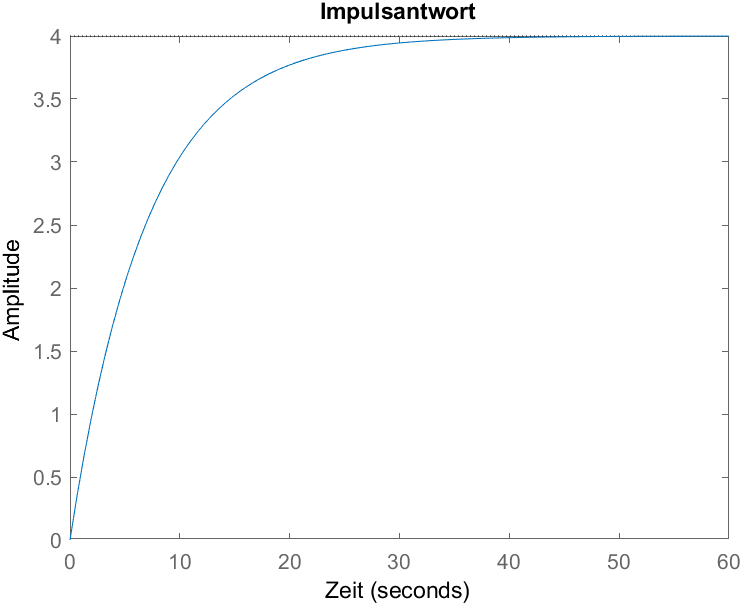
\includegraphics[width=0.8\textwidth]{{diagrams/impulseantwort.png}}
	\caption[Impulsantwort]{Impulsantwort}
	\label{fig:impulse}
\end{figure}